
L'hypothèse de recherche est basée sur la conception et la réalisation en technologie CMOS d'une référence de tension intégrée innovante qui soit rendue tolérante au débit de dose en environne-ment radiatif sévère, ceci en utilisant la technique de drainage des photo-courants induits.

Effet des radiations sur les circuits électroniques
Dans la majorité des cas, pour s’assurer du bon fonctionnement d’un circuit électronique, réfé-rence de tension ou non, on leur fait subir des tests en simulation. Ces tests permettent de prédire si le circuit fonctionnera indépendamment : de la répétabilité imparfaite de fabrication (Process), de la tension d’alimentation (Voltage) et de la température de fonctionnement (Temperature). Ces tests sont donc qualifiés de "PVT".

Certains circuits électroniques sont destinés à fonctionner dans des environnements plus agressifs que d’autres, c’est notamment le cas des circuits qui équipent les systèmes opérant aux abords de centrales nucléaires. Dans ce type d'environnement, les circuits sont soumis à des radiations qui peuvent perturber leur fonctionnement, aux tests PVT est alors ajouté le test aux radiations, dit R pour Radiation.
On distingue deux types de dégradations des circuits électroniques soumis à des radiations : d’une part, ceux induits par la dose, cumulée au cours du temps, d’autre part, ceux induits par le débit de dose qui impacte le circuit de manière quasi-instantanée.

Dose de radiation :
La dose de radiation fait référence à la quantité totale de rayonnement absorbée par un compo-sant électronique sur une période prolongée. Cette exposition prolongée peut résulter de diverses sources, telles que des environnements spatiaux, des applications médicales ou des installations de recherche nucléaire. Les dommages causés par la dose de radiation sont souvent cumulatifs et dépendent de la sensibilité du composant électronique spécifique ainsi que de la nature du rayon-nement. Les effets peuvent se manifester sous forme de perturbations électriques, de dégradation des matériaux ou même de défaillance complète du circuit.

Débit de dose de radiation :
Contrairement à la dose de radiation, qui est accumulée au fil du temps, le débit de dose caracté-rise le flux instantané de radiation. Il peut s'agir d'une exposition soudaine et intense à des radia-tions ionisantes, comme celles rencontrées lors d'événements tels que des tempêtes solaires ou des explosions nucléaires.
Les effets du débit de dose de radiation sont souvent plus immédiats et peuvent provoquer des perturbations temporaires ou permanentes dans le fonctionnement des circuits électroniques. Cela peut se traduire par des erreurs de données, des dysfonctionnements temporaires ou une défaillance complète du composant.
La mesure du débit de dose est généralement exprimée en Gray par seconde (Gy/s), en Sievert par seconde (Sv/s) ou encore en rad/s  , indiquant la quantité de rayonnement absorbée par unité de temps.
Ces deux modes de dégradation sont importants à considérer lors de la conception et de l'utilisa-tion de composants électroniques dans des environnements exposés à des radiations, tels que l'es-pace, les installations nucléaires ou les applications médicales. Des techniques de conception et des matériaux spécifiques peuvent être utilisés pour atténuer les effets des radiations et garantir la fiabilité et la durabilité des circuits électroniques dans de telles conditions.

Jonctions PN et radiation
Les effets du débit de dose se concentrent principalement sur les jonctions PN. En effet, lors de l'irradiation, les jonctions PN se comportent comme des générateurs de courants .
Dans les technologies les plus standards dites "bulk" les transistors sont directement fabriqués dans le substrat. Cette méthode de fabrication est rapide, peu couteuse et adoptée par la grande majorité des fabricants de circuits intégrés. Un inconvénient de ce mode de fabrication est qu'il laisse peu, voire aucune, latitude pour ajuster les paramètres des transistors une fois le circuit fabriqué – même s’il est vrai qu’il existe des techniques dites de body-biasing qui permettent d’agir avec une faible marge de manœuvre sur les caractéristiques des transistors. Heureuse-ment, certains fabriquant de circuits intégrés proposent des circuits basés sur des technologies dites FD-SOI (Fully Depleted - Silicon On Insulator). Dans ces technologies, un isolant sépare les transistors du substrat en silicium, les transistors sont alors fabriqués dans une fine couche de sili-cium sans porteurs de charges. Le principal intérêt de cette technologie est la Back-Gate (grille arrière), une connexion qui permet de polariser le silicium qui se trouve sous l'oxyde enterré, agissant ainsi comme une seconde grille (Gate) et permettant de modifier significativement les performances des transistors.
Les deux technologies sont présentées à la Figure 1.

\begin{figure}
    \centering
    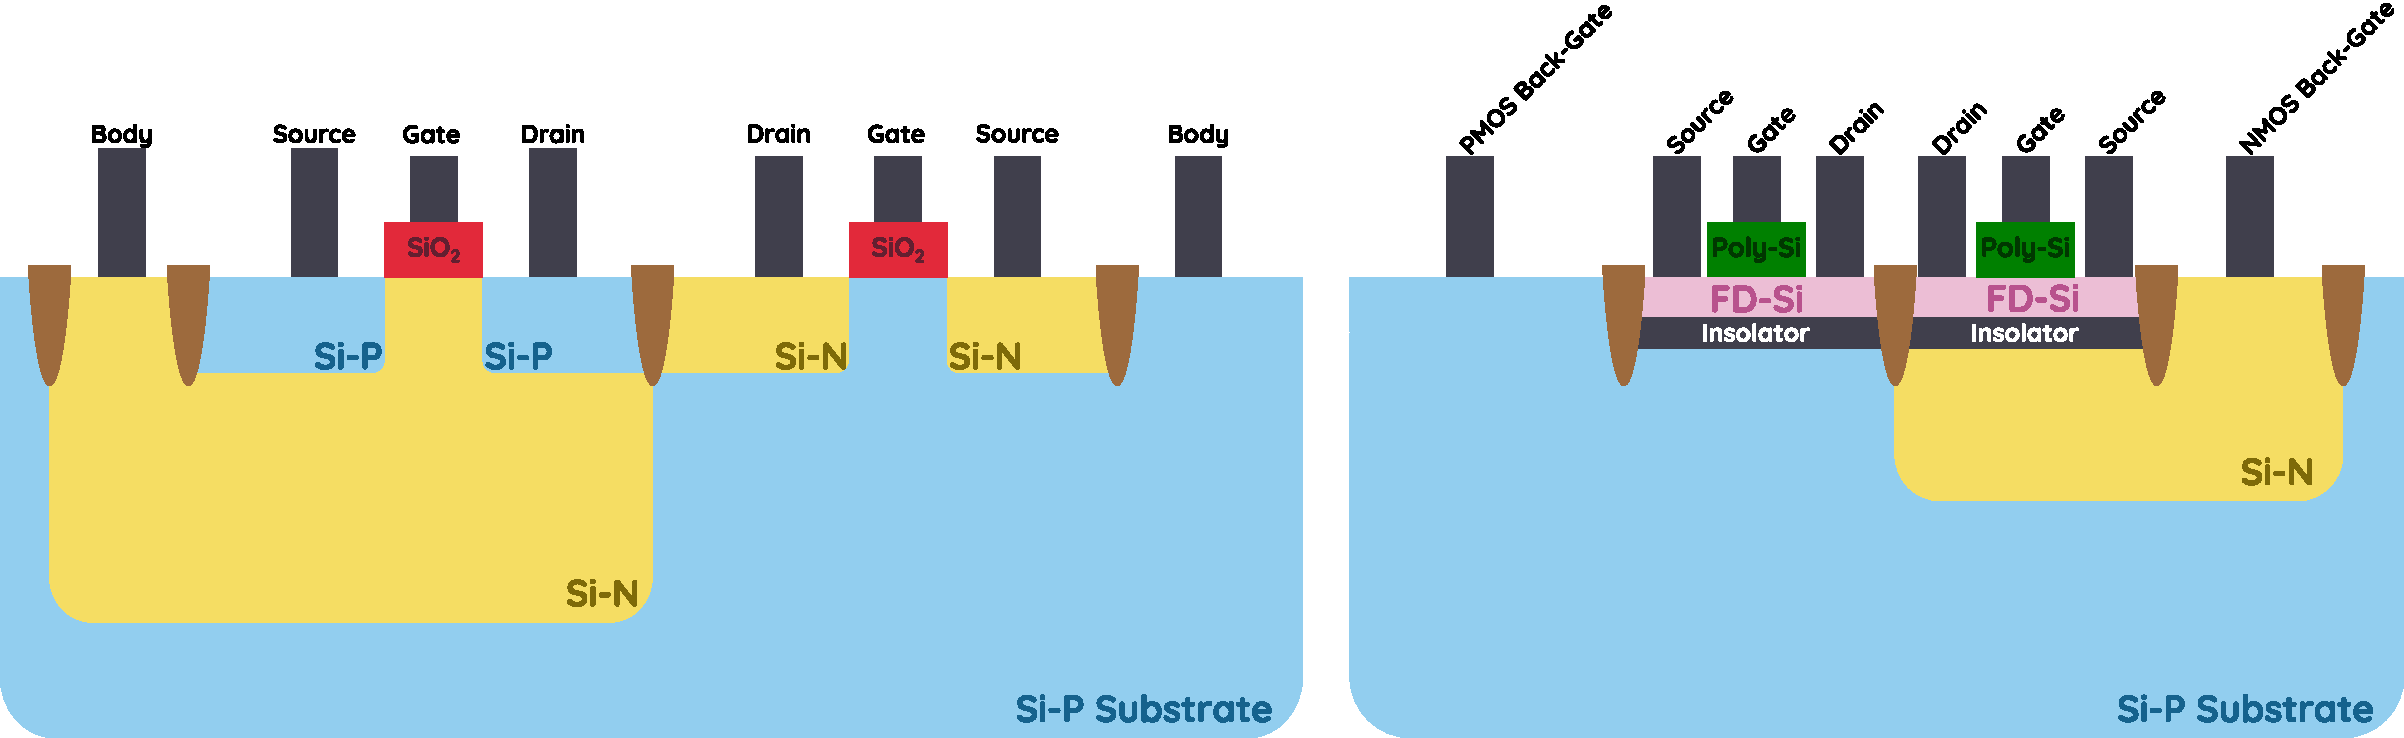
\includegraphics[width=0.7\textwidth]{figures/FabBulkVsFdsoi.pdf}
    \caption{Vue en coupe d'une technologie Bulk (à gauche) face à une technologie FD-SOI (à droite)}
    \label{fig:bulk_vs_fdsoi}
\end{figure}
 

Au point de vue des radiations, en termes de tenue au débit de dose, la technologie est par nature plus robuste : en effet, le caractère Fully Depleted du canal des transistor et le nombre réduit de jonctions PN diminue drastiquement les courants générés lors d'une irradiation. Au niveau de la dose, les grilles poly-Si de la FD-SOI collectent moins de charges que les grilles SiO2 des technolo-gies bulk. De plus, le contrôle de la Back-Gate permet, dans une certaine mesure de compenser la chute des tensions de seuil induite par les radiations.

\begin{metsUneSource}
milieu déja écrit
\end{metsUneSource}


\section{Introduction}

L'hypothèse de recherche est basée sur la conception et la réalisation en technologie CMOS d'une référence de tension intégrée innovante qui soit rendue tolérante au débit de dose en environnement radiatif sévère, ceci en utilisant la technique de drainage des photo-courants induits.

\section{Effet des radiations sur les circuits electroniques}

Dans la majorité des cas, pour s’assurer du bon fonctionnement d’un circuit électronique, référence de tension ou non, on leur fait subir des tests en simulation. Ces tests permettent de prédire si le circuit fonctionnera indépendamment : de la répétabilité imparfaite de fabrication (\textit{Process}), de la tension d’alimentation (\textit{Voltage}) et de la température de fonctionnement, (\textit{Temperature}). Ces tests sont donc qualifiés de "PVT".

\begin{metsUneSource}
“Process-Voltage-Temperature Analysis of a CMOS-MEMS Readout Architecture” explique bien les pvt
\end{metsUneSource}

Certains circuits électroniques sont destinés à fonctionner dans des environnements plus agressifs que les autres, c’est notamment le cas des circuits qui équipent les systèmes opérant aux abords de centrales nucléaires ou encore des circuits présents dans les satellites artificiels. Dans ces environnements, les circuits sont soumis à des radiations qui peuvent perturber leur fonctionnement, aux tests PVT est alors ajouté le test R pour Radiation.
On distingue deux modes de dégradations des circuits électroniques par des radiations :

\begin{metsUneSource}
  2 modes de dégradation
\end{metsUneSource}

La dose, qui se fait par une exposition prolongée d’un circuit face à des radiations et qui augmente avec le temps ; le débit de dose qui impact le circuit de manière instantané et en un temps donné.

\subsection{Dose}

La dose de radiation fait référence à la quantité totale de rayonnement absorbée par un composant électronique sur une période prolongée. Cette exposition prolongée peut résulter de diverses sources, telles que des environnements spatiaux, des applications médicales ou des installations de recherche nucléaire. Les dommages causés par la dose de radiation sont souvent cumulatifs et dépendent de la sensibilité du composant électronique spécifique ainsi que de la nature du rayonnement. Les effets peuvent se manifester sous forme de perturbations électriques, de dégradation des matériaux ou même de défaillance complète du circuit.

\begin{metsUneSource}
Débit de dose de radiation :
\end{metsUneSource}

Contrairement à la dose de radiation, qui est accumulée au fil du temps, le débit de dose fait référence à la quantité de rayonnement absorbée par un composant électronique en un laps de temps donné. Il peut s'agir d'une exposition soudaine et intense à des radiations ionisantes, comme celles rencontrées lors d'événements tels que des tempêtes solaires ou des explosions nucléaires.
Les effets du débit de dose de radiation sont souvent plus immédiats et peuvent provoquer des perturbations temporaires ou permanentes dans le fonctionnement des circuits électroniques. Cela peut se traduire par des erreurs de données, des dysfonctionnements temporaires ou une défaillance complète du composant.

La mesure du débit de dose est généralement exprimée en Gray par seconde (Gy/s), en Sievert par seconde (Sv/s) ou encore en rad par seconde (rad/s) qui est ancienne unité mais qui est encore utilisée dans les differents papier et écrits scientifiques, indiquant la quantité de rayonnement absorbée par unité de temps.
Ces deux modes de dégradation sont importants à considérer lors de la conception et de l'utilisation de composants électroniques dans des environnements exposés à des radiations, tels que l'espace, les installations nucléaires ou les applications médicales. Des techniques de conception et des matériaux spécifiques peuvent être utilisés pour atténuer les effets des radiations et garantir la fiabilité et la durabilité des circuits électroniques dans de telles conditions.

\begin{metsUneSource}
  Etat de l’art dose
\end{metsUneSource} 


\subsection{Débit de dose}

\begin{metsUneSource}
SC rogers
Photo courant
ELDRS
Jonctions PN

Radiation-Induced Prompt Photocurrents in Microelectronics: Physics
\end{metsUneSource}

\begin{metsUneSource}
 1) 
\end{metsUneSource}
           
\subsubsection{ Valeurs de débit}

\begin{figure}[H]
  \centering
  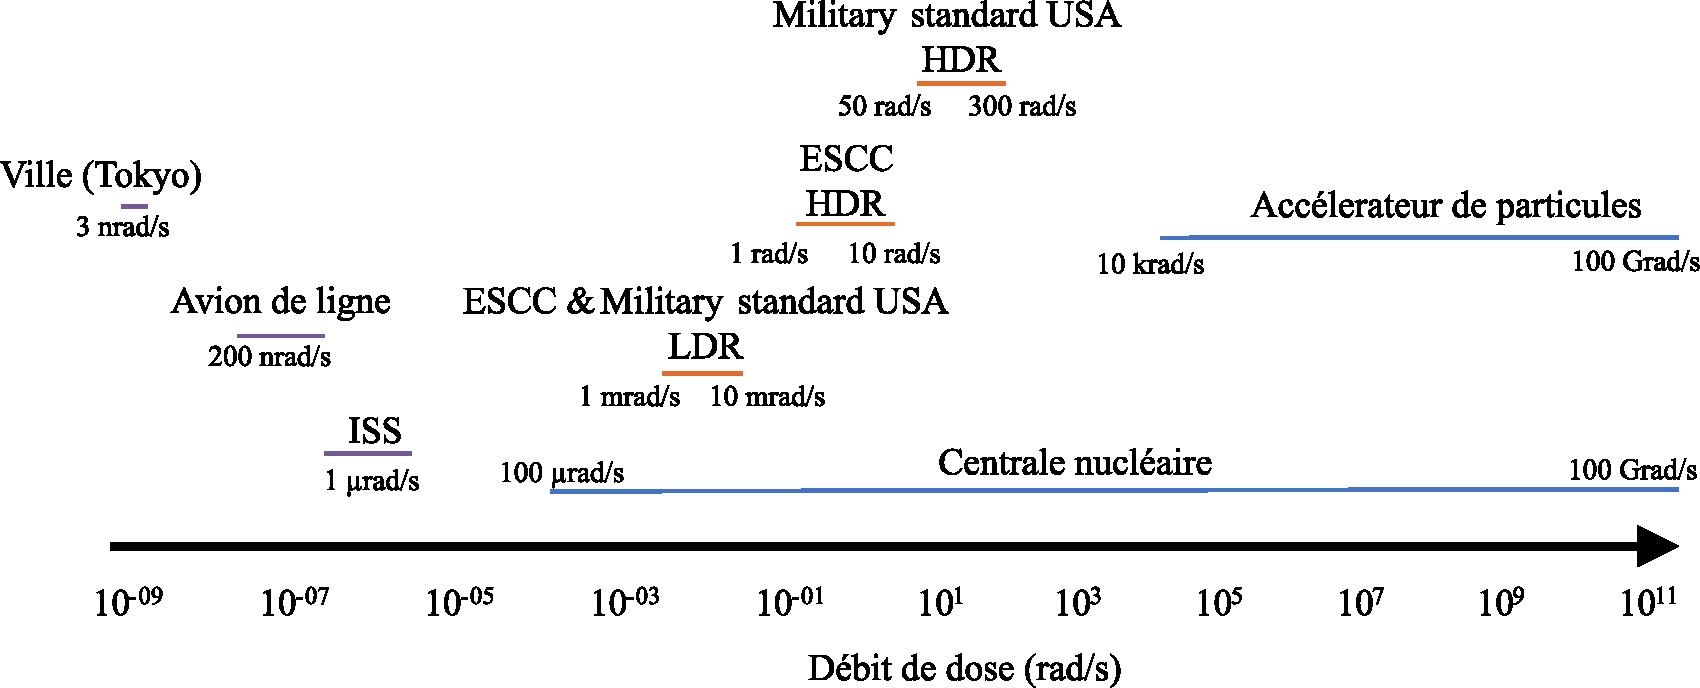
\includegraphics[width=0.7\textwidth]{figures/DoseRateExemple.pdf}
  \caption{Recapitulatif des valeurs de débit de dose dans des situations courantes.}
  \label{fig:DoseRateExemple}
\end{figure}

\subsection{ Considération du bon mode de dégradation}

\begin{metsUneSource}
ça n'est pas n'importe où que le peut avoir des debits si fort avec une dose négligeable
\end{metsUneSource}

\begin{metsUneSource}
Ipp vs effet dose
\end{metsUneSource}

\section{Développement d’un circuit robuste aux radiations}
\subsection{Choix d’une technologie polyvalente avec des ambitions de robustesse face aux raditions}

Le choix de la technologie des semi-conducteurs est un facteur crucial pour la réalisation d'une référence de tension désensibilisée au débit de dose. Dans le cadre de cette étude, le choix s’est porté sur technologie dont le comportement face aux radiations est déjà réputé comme étant bon, et dont certaines fonctionnalités peuvent aider à la compensation des troubles engendrés par les radiations.


\begin{metsUneSource}
Source 28 fdsoi déjà un bon client


Very small volume of charge collection ion-induced charges only collected from Si film not below Buried Oxide (BOX), not beyond STI Best radiation isolation vs. other technologies no multiple charge collections nor SEL weakness as for FinFET Latchupimmunity with buried oxide layer (BOX) and secured for bulk areas BOX thinning in FDSOI creates new TID balance no inter-device leakage VTH shift on front gate self-recovered stronger coupling between interfaces

philippe roche
\end{metsUneSource}



L’études est donc réalisée sur la technologie \textbf{28nm FD-SOI} (\textit{Fully Depleted Silicon On Insulator}) du fondeur STMicroelectronics dont l’architecture permet l’absence de porteurs dans le canal, et donc de jonction PN dans le canal des transistors, ce qui, devrait réduire drastiquement l’apparition de courants parasites dans cette zone (pas de jonction PN).

\begin{metsUneSource}
FDSOI c’est déplété
Photo transistor
\end{metsUneSource}



Aussi, l’architecture de la technologie FD-SOI, presentée dans la figure Fig.%\ref*{fig:SOIvsBULK}
, permet, à l’inverse des technologies \textit{Bulk}, un control fin de la tension de seuil des transistors atteint en polarisant le silicium présent sous les transistors appelé "\textit{Back-Gate}".

\begin{figure}[H]
  \centering
  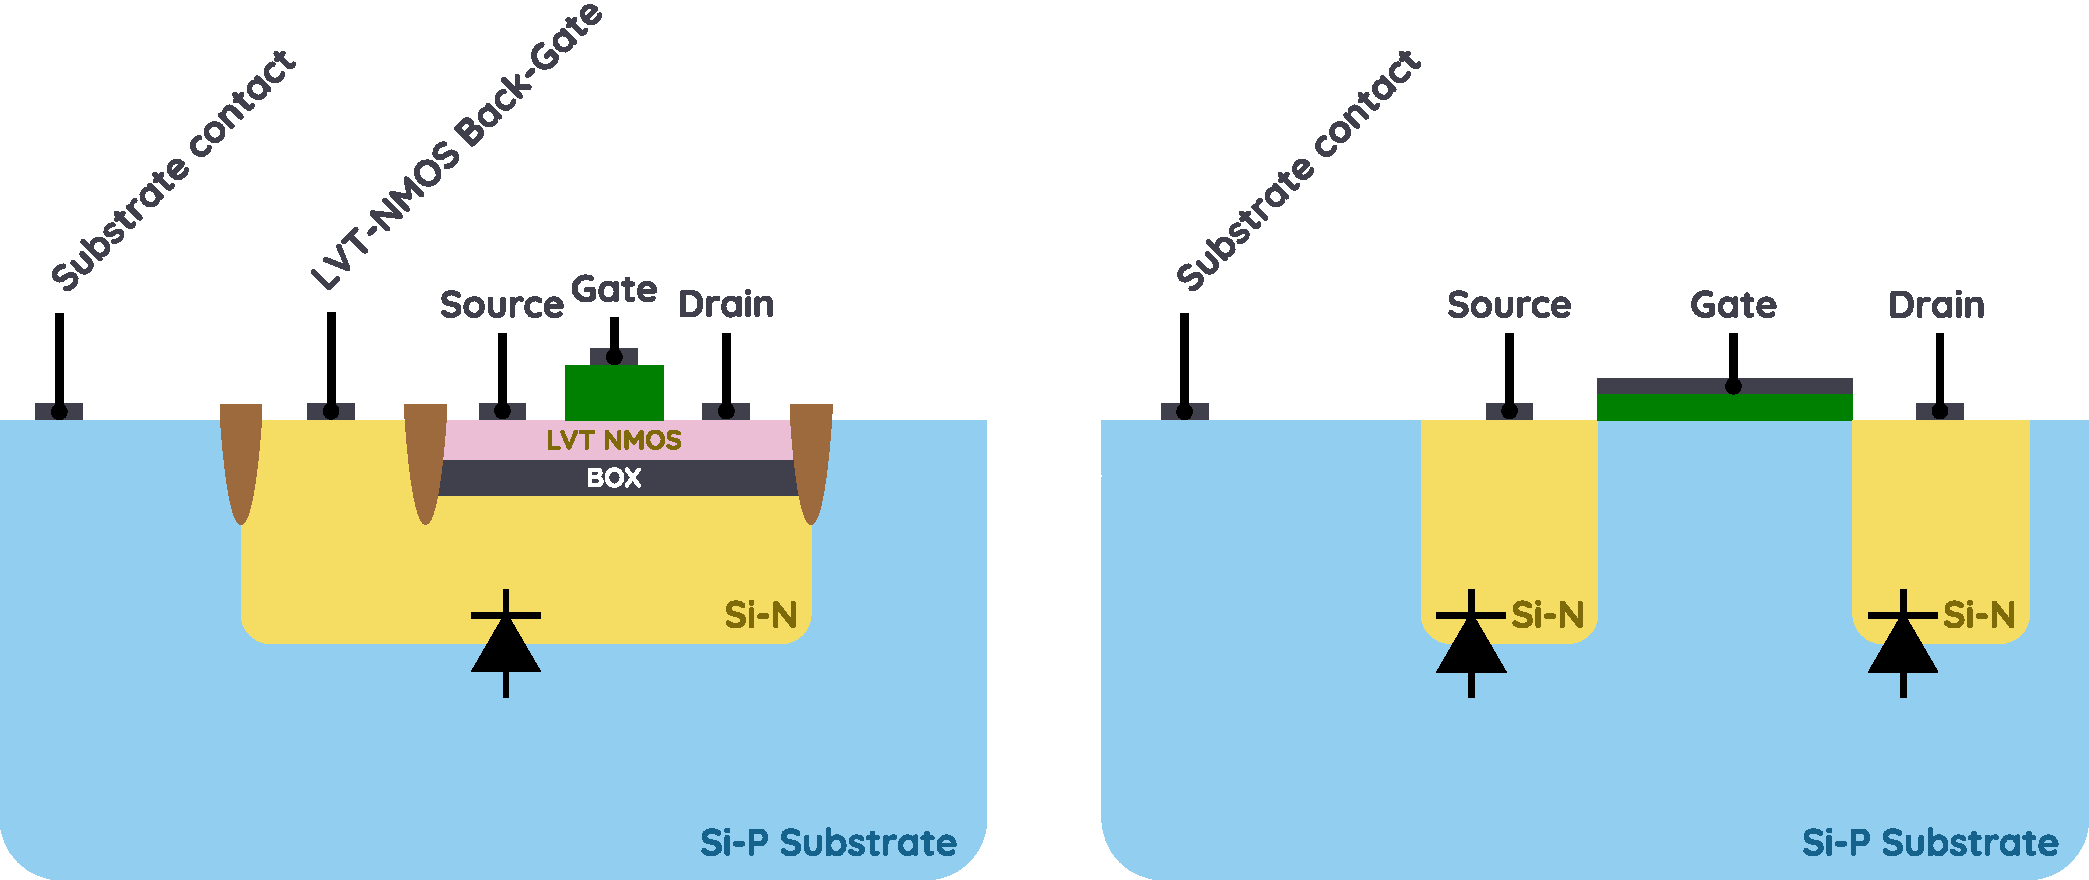
\includegraphics[width=0.9\textwidth]{figures/SOIvsBULK.pdf}
  \caption{Comparaison des topologie \textit{FD-SOI} (à gauche) et \textit{Bulk} (à droite).}
  \label{fig:SOIvsBULK}
\end{figure}
\begin{metsUneSource}
Back Gate VS \textit{Bulk}
\end{metsUneSource}

La \textit{Back-Gate}, une fois polarisée, aporte de la flexibilité quant au comportement des transistors, notamment au niveau de leur tension de seuil, Fig %\ref{fig:VTvsVBB},
 une flexibilité inatteignable en \textit{Bulk} sans modifier la taille des transistors. La polarisation de la \textit{Back-Gate} est une technique similaire au \textit{Bulk-Body-Biasing} mais avec des perfomances bien plus élevées et des problèmes intrinsèques au \textit{Bulk} en moins.

\begin{figure}[H]
  \centering
  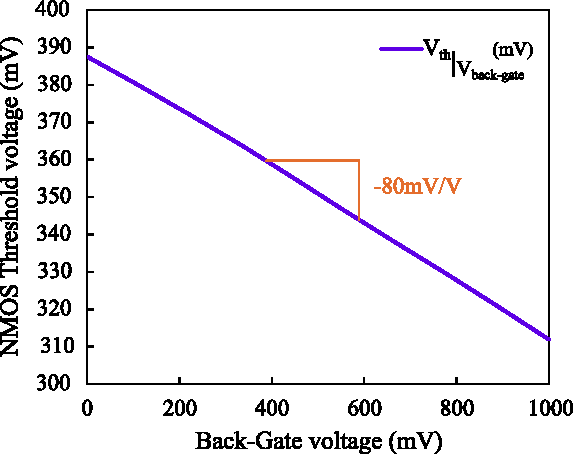
\includegraphics[width=0.5\textwidth]{figures/Vt(Vbb).pdf}
  \caption{Evolution de la tension de seuil en fonction de la tension de \textit{Back-Gate} (VBB).}
  \label{fig:VTvsVBB}
\end{figure}

\begin{metsUneSource}
The 4th terminal encore Back Gate VS bulk
\end{metsUneSource}

Toutefois l’utilisation de la \textit{Back-Gate} implique l’utilisation de jonctions PN dans le substrat du circuit. Ces jonctions permettent de modifier la tension de la \textit{Back-Gate} sans modifier la tension de tout du substrat, en effet, une jonction PN polarisée en sens inverse ne laissant pas passer de courant, il est donc possible d’augmenter la tension d’un puit N, la \textit{Back-Gate}, sans modifier la tension de substrat.
L’apparition de ces jonctions PN dégrade le comportement du circuit face aux radiations en generant des courants parasites sous les transistors ce qui modifie la tension de leur \textit{Back-Gate} et donc, par extension, leur tension de seuil. La gestion des courants parasites générés est donc un enjeu majeur pour la réalisation d’un circuit robuste face aux radiations, l'une des solutions possible est de drainer ces courants, cette solution est présentée dans la section %\ref*{sec:drainage}.

\begin{metsUneSource}
……………… courant parasite, évacuation par l’alim mais pas par le reste sur circuit (CR sur la bg)
\end{metsUneSource}




\subsection{Référence de tension}

Une référence de tension est un circuit électronique qui permet de générer une tension connue et qui se veut, dans le meilleur des cas, constante en toutes circonstances. 

\begin{metsUneSource}
Source ref tension


shema 80ppm/°C
\end{metsUneSource}



\subsection{Amplificateur opérationnel}




